\chapter{Preliminari}
In questo capitolo verranno presentati alcuni degli argomenti preliminari necessari alla realizzazione della tesi.\\
Nella sezione 1.1 viene delineato il contesto riguardante l'ambito del Machine Learning, presentando gli argomenti di questo campo di studi che riguardano questa tesi. Nella sezione 1.2 si presenta l'attuale stato dell'arte riguardo le Reti Neurali Ricorrenti, gli strumenti a disposizione e alcune future possibili applicazioni degli argomenti trattati in questa tesi.

\section{Contesto}
In un mondo sempre più interconnesso e in rapida evoluzione, gli approcci statici al Machine Learning possono diventare impraticabili quando si tratta di produrre sistemi in grado di adattarsi dinamicamente allo stato fisico e mentale degli utenti che vi interagiscono. Inoltre, con l'ampia diffusione di dispositivi in grado di raccogliere in tempo reale informazioni sulla condizione attuale degli utenti, sono costantemente resi a disposizione nuovi dati con cui perfezionare i modelli di Machine Learning in uso attraverso tecniche di Addestramento Continuo.

\subsection{Human State Monitoring}
Uno di questi contesti è lo \textit{Human State Monitoring}. Con questo termine si indica l'obiettivo di un sistema di raccogliere dati riguardanti l'attuale stato psico-fisico di un individuo e trarre conclusioni sulla sua condizione attuale, ad esempio interpretando un battito cardiaco elevato insieme ad un alto livello di sudorazione come uno stato di stress, o determinati movimenti facciali come una condizione di sonnolenza. L'avere a disposizione metodologie efficienti nel catalogare queste condizioni umane può portare a sistemi responsivi e adattivi, che modificano le proprie interfacce o i propri comportamenti accomodando lo stato psico-fisico attuale dell'utente.\\\\
Un possibile applicazione dello \textit{Human State Monitoring} la si può trovare nel progetto europeo TEACHING$^{\cite{teaching2020}}$, che mira alla produzione di un toolkit per costruire applicazioni autonome efficienti che facciano uso di intelligenza simile a quella umana. L'obiettivo di questo toolkit è supportare lo sviluppo e il rilascio di applicazioni che possano sfruttare il feedback umano per ottimizzare, personalizzare e guidare il modo in cui esse forniscono i propri servizi. In altre parole, applicazioni che sfruttino lo \textit{Human State Monitoring} per adattarsi dinamicamente alle condizioni dell'utente in tempo reale.\\
Per poter realizzare questo adattamento continuo è necessario, oltre al flusso di dati in tempo reale sullo stato corrente dell'utente, anche un sistema che sappia efficientemente e correttamente interpretare questi dati, traendo conclusioni sulle attuali condizioni della persona. Questa situazione presenta le classiche caratteristiche necessarie all'applicazione del Machine Learning: abbiamo dati raccolti da sensori che possono essere difettosi, per cui i dati possono contenere incertezze o essere rumorosi o incompleti, ed essendo in esame lo stato umano è molto difficile, se non impossibile, formalizzare attraverso una descrizione procedurale la classificazione di questi dati in categorie comportamentali, ad esempio affaticamento o sonnolenza.

% breve introduzione al mondo dell'addestramento Machine Learning per introdurre i concetti fondamentali per la tesi
\subsection{Addestramento} L'addestramento di un modello di Machine Learning avviene attraverso l'utilizzo di un insieme di dati chiamato \textit{training set}, che contiene i dati di addestramento. Questi dati sono sottoposti al modello, che li userà nelle sessioni di addestramento. Nell'addestramento supervisionato, il training set è composto da una serie di esempi composti da coppie $\langle$input, etichetta$\rangle$ dove le etichette sono fornite da chi ha preparato il training set, detto supervisore. Queste etichette vengono assegnate agli input in base ad una certa funzione $f$, che è ignota ed è la funzione che il modello di Machine Learning deve apprendere. Il modello elabora questi dati e le loro etichette cercando di apprendere quali etichette sono assegnate a quali dati e in che modo. L'obiettivo del modello è quindi trovare una buona approssimazione di $f$ che faccia corrispondere le etichette corrette ai rispettivi input.\\
Per verificare l'apprendimento, si sottopone al modello addestrato dei dati non etichettati, denominati \textit{test set}, e si verificano le etichette che il modello assegna a tali dati controllando se ha classificato correttamente o meno. La percentuale di dati correttamente etichettati dal modello è chiamata \textbf{accuratezza}.

\subsection{Loss} Per misurare l'andamento dell'apprendimento di un modello di Machine Learning, vengono usate funzioni che vanno a valutare il modello in base alle risposte che esso fornisce sui dati etichettati, confrontandole con le etichette reali. Queste funzioni prendono il nome di funzioni di \textit{loss}. Ne esistono di diversi tipi, a seconda del problema in esame: ad esempio, nei problemi dove ad ogni input va assegnata una risposta si/no (classificazione binaria) una loss molto usata è la cross-entropia binaria (\textit{binary crossentropy}), delineata nell'equazione \ref{eq:bin_crossentr} dove $y$ è l'etichetta reale, che può assumere valori 0/1, falso/vero o altri, e $p(y)$ è la probabilità assegnata dal modello in fase di previsione.
\begin{equation}\label{eq:bin_crossentr}
H_p(q) = -\frac{1}{N}\sum_{i=1}^N \left(y_i\cdot\log(p(y_i)) + (1 - y_i)\cdot\log(1 - p(y_i))\right)
\end{equation}

\subsection{Reti Neurali} In letteratura vengono studiati moltissimi modelli di Machine Learning. Si va dai più semplici come i modelli lineari, nei quali abbiamo un'equazione nella forma $y = w_0x + w_1$ e dobbiamo apprendere i $w_0$ e $w_1$ che ai dati $x$ fanno corrispondere le corrette etichette $y$, alle \textit{Support Vector Machine}, che cercano di trovare dei confini di divisione fra insiemi di dati così da poterli classificare.\\
Un'ampia area di modelli di Machine Learning è quella delle cosiddette \textbf{reti neurali}, studiate sin dagli anni '40. Esse prendono liberamente spunto dalla struttura dei neuroni del cervello umano (Figura \ref{fig:neurone}), che sono stati schematizzati in strutture matematiche denominate \textbf{perceptron}$^{\cite{rosenblatt1958perceptron}}$.
\begin{figure}[h]
	\begin{center}
		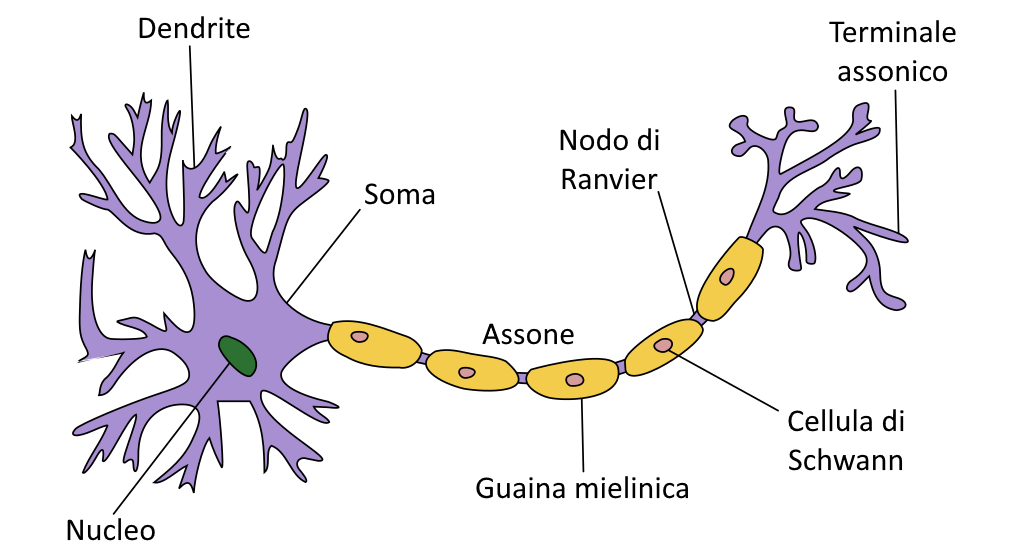
\includegraphics[width=0.75\textwidth]{img/neurone.png}
		\caption{Neurone (credits: Quasar, Wikipedia)}
		\label{fig:neurone}
	\end{center}
\end{figure}
In un perceptron (Figura \ref{fig:perceptron}), ad ogni input $x_i$ è assegnato un peso $w_i$ che lo rende più o meno importante nel contribuire al risultato $y$, che viene calcolato dal nodo attraverso la \textbf{funzione di attivazione}, nella forma \ref{eq:act_fun} dove $b$ è un ulteriore peso definito \textit{bias}.\\\\
\begin{equation}\label{eq:act_fun}
f\left(\sum_i w_i\cdot x_i + b\right)
\end{equation}
\begin{figure}[h]
	\begin{center}
		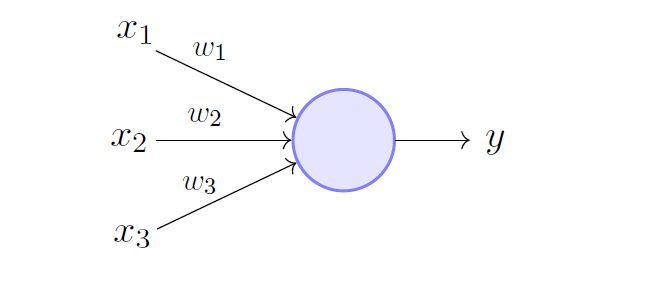
\includegraphics[width=0.5\textwidth]{img/perceptron.png}
		\caption{Perceptron}
		\label{fig:perceptron}
	\end{center}
\end{figure}
Una rete neurale (Figura \ref{fig:reteneurale}) è composta da un insieme di perceptron collegati fra loro suddivisi su livelli, o \textit{layer}: una rete neurale composta da un elevato numero di layer è detta profonda, o \textit{deep neural network}, e i layer interni sono detti layer nascosti.
\begin{figure}[h]
	\begin{center}
		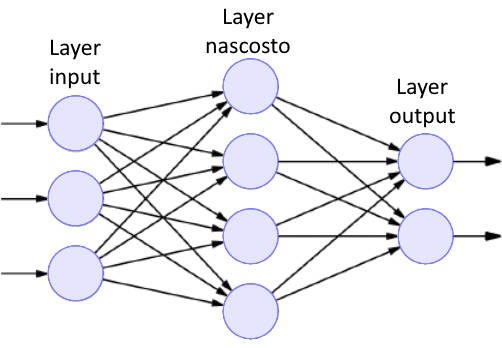
\includegraphics[width=0.75\textwidth]{img/reteneurale.jpg}
		\caption{Esempio di rete neurale (credits: databricks.com)}
		\label{fig:reteneurale}
	\end{center}
\end{figure}
\\\\
Le funzioni di attivazione possono essere funzioni di qualsiasi tipo, ma le più usate e studiate sono funzioni specifiche come ReLU e softmax. La funzione ReLU (\textit{Rectified Linear Unit}) è molto semplice e veloce da calcolare: restituisce la parte positiva del proprio input, e consente un migliore apprendimento nelle reti neurali profonde$^{\cite{pmlr-v15-glorot11a}}$.
\begin{equation}\label{eq:fun_relu}
ReLU(x) = max(0, x)
\end{equation}
La funzione softmax, invece, prende in input un vettore di $K$ valori e lo comprime in un vettore sempre di $K$ elementi ma dai valori compresi nell'intervallo $(0, 1)$ e la cui somma è 1. Vengono usate nel layer finale delle reti neurali realizzate per compiti di classificazione: ogni valore $\sigma(\textbf{z})_j$  è interpretabile come la probabilità che l'input appartenga alla classe $j$ fra le $K$ possibili.
\begin{equation}\label{eq:fun_softmax}
\sigma(\textbf{z})_j = \frac{e^{z_j}}{\sum_{k=1}^K e^{z_k}}\:\:\:\:\mbox{ per }j = 1,\ldots,K
\end{equation}
Le funzioni di attivazione descrivono quindi il comportamento dei nodi di una rete neurale e la scelta della funzione di attivazione è un elemento importante nella strutturazione di una rete neurale.
\subsubsection{Tipologie} La struttura interna di una rete neurale influenza particolarmente i risultati che essa può ottenere. A seconda del problema che si vuole risolvere, si può rendere necessario l'utilizzo di reti neurali con strutture interne complesse, in modo da ottenere risultati soddisfacenti. In particolare, in letteratura attualmente alcune delle strutture più studiate sono (Figura \ref{fig:tipologiereti}):
\begin{itemize}
    \item[-] Reti Feed Forward (FF)$^{\cite{0471349119}}$
    \item[-] Reti Neurali Ricorrenti (RNN, Recurrent Neural Networks)$^{\cite{10.1162/neco.1997.9.8.1735}}$
    \item[-] Auto Encoders (AE)$^{\cite{DBLP:journals/corr/abs-2003-05991}}$
    \item[-] Reti Profonde Convolutive (DCN, Deep Convolutional Networks)$^{\cite{DBLP:journals/corr/abs-2011-12960}}$
    \item[-] Echo State Networks (ESN)$^{\cite{GALLICCHIO201833}}$
\end{itemize}
Alcune di queste strutture ottengono risultati particolarmente buoni su certe tipologie di problemi: ad esempio, le DCN possiedono una struttura ispirata alla corteccia visiva del cervello e sono particolarmente usate nel campo del riconoscimento delle immagini e del linguaggio parlato, mentre le RNN mantengono informazioni riguardo gli input precedenti e consentono di modellare i comportamenti dinamici e ricorrenti delle sequenze temporali.
\begin{figure}[h]
	\begin{center}
		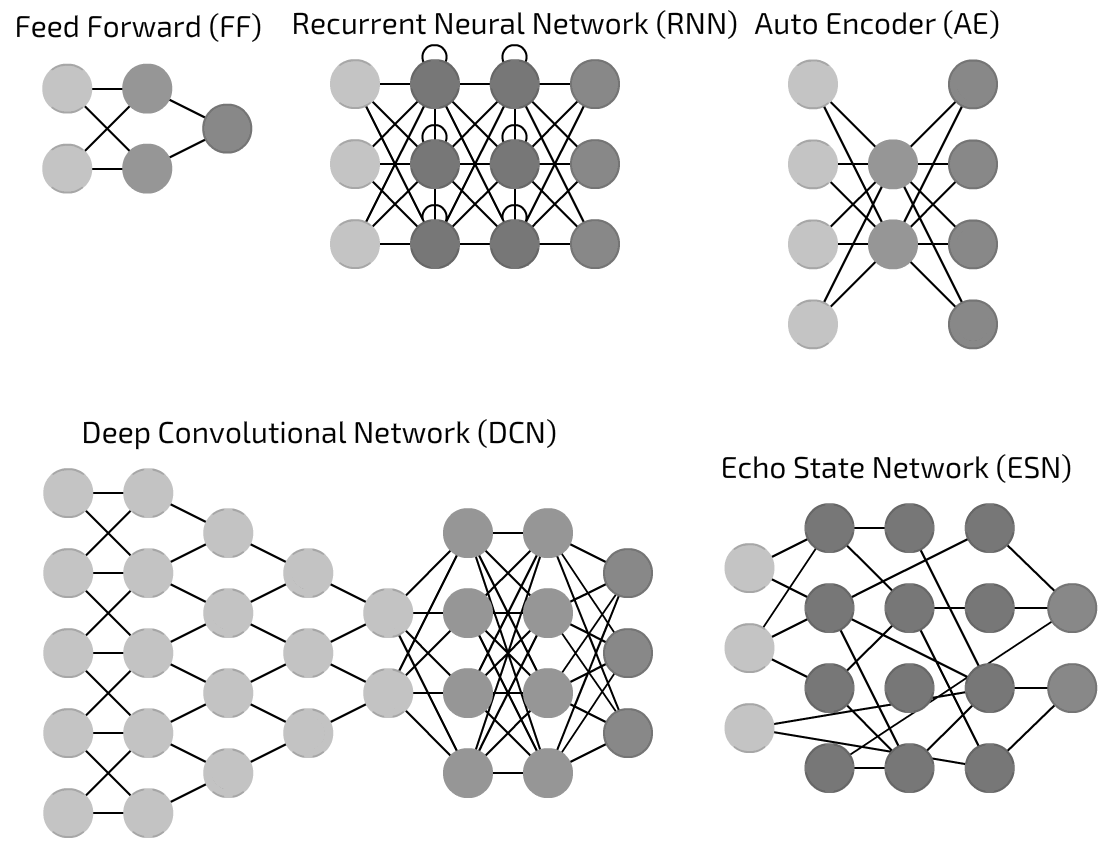
\includegraphics[width=0.85\textwidth]{img/tipologiereti.png}
		\caption{Esempi di reti neurali (credits: Andrew Tch, towardsdatascience.com)}
		\label{fig:tipologiereti}
	\end{center}
\end{figure}

\subsubsection{Backpropagation} La retropropagazione dell'errore, \textit{backward propagation of errors}$^{\cite{Rumelhart_1986}}$, è l'algoritmo più diffuso per l'addestramento supervisionato delle reti neurali. Questo algoritmo consiste di due fasi:
\begin{itemize}
    \item[-] \textit{Forward phase}, dove gli input vengono elaborati dalla rete neurale fino a produrre un output
    \item[-] \textit{Backward phase}, dove l'output prodotto è confrontato con la vera etichetta assegnata e, attraverso calcoli differenziali, vengono individuati i contributi all'errore di ogni nodo. Con questi contributi, attraverso un algoritmo di ottimizzazione (solitamente, la discesa di gradiente), vengono modificati i pesi delle connessione fra i nodi, partendo dai nodi output e risalendo la rete fino ai nodi input.
\end{itemize}
Questo algoritmo richiede quindi che le funzioni di attivazione dei nodi siano differenziabili, e può soffrire di un problema che prende il nome di \textit{vanishing/exploding gradient problem}$^{\cite{DBLP:journals/corr/abs-1211-5063}}$, o problema della scomparsa/esplosione del gradiente. Nel dettaglio, attraverso questo algoritmo ogni parametro del modello viene modificato, durante la \textit{backward phase}, in maniera proporzionale alla derivata parziale della funzione \textit{loss} rispetto al parametro stesso. Propagando all'indietro attraverso la regola della catena$^{(\ref{eq:catena})}$ dei gradienti compresi nell'intervallo $[0, 1]$, come nel caso di alcune funzioni di attivazione, il prodotto diventa tanto più piccolo quanto più è profonda la rete neurale o, viceversa, esplodere in caso di gradienti dai valori elevati.
\begin{equation}\label{eq:catena}
D\left[f(g(x))\right] = f'(g(x))\cdot g'(x)
\end{equation}
Questo problema viene mitigato dall'uso di funzioni di attivazioni diverse, come le già citate ReLU$^{(\ref{eq:fun_relu})}$ e softmax$^{(\ref{eq:fun_softmax})}$, o dall'uso di algoritmi di addestramento che fanno uso solo del segno del gradiente e non della sua norma, come l'algoritmo Rprop$^{\cite{Riedmiller92rprop-}}$.\\
Nelle reti neurali ricorrenti, un grande contributo alla mitigazione del problema è avvenuto grazie all'introduzione delle LSTM, \textit{Long Short-Term Memory}$^{\cite{10.1162/neco.1997.9.8.1735}}$, che mantengono informazioni sullo stato del modello senza propagarle attraverso funzioni non lineari.

\subsection{Continual Learning} L'addestramento di un modello di Machine Learning attraverso un \textit{training set} disponibile fin da subito e fornito interamente al modello è denominato "addestramento \textit{offline}", o \textit{offline training}. Esistono contesti, però, dove i dati necessari o utili all'addestramento non sono subito tutti disponibili, ma diventano tali col passare del tempo. Un esempio di questa situazione sono i sistemi di raccomandazione in servizi come Netflix o YouTube: essi imparano continuamente i gusti dell'utente, in modo da fornire suggerimenti su video e film sempre adatti ai gusti del momento. Questa situazione, in cui i dati di addestramento diventano disponibili col passare del tempo e cioè di addestramento continuativo, è detta "Addestramento Continuo", o \textit{continual learning}.\\
Nel caso dell'Addestramento Continuo, un grosso ostacolo è quello denominato \textit{catastrophic forgetting}$^{\cite{MCCLOSKEY1989109}}$: quando una rete neurale già addestrata viene addestrata su nuovi dati, essa tenderà a dimenticare ciò che ha appreso sui dati precedenti. Questa situazione è una manifestazione del cosiddetto dilemma della \textbf{plasticità-stabilità}: si ha stabilità quando la nuova conoscenza non interferisce con la vecchia conoscenza, mentre si parla di plasticità quando la nuova conoscenza migliora la conoscenza già appresa e viceversa. Questi due obiettivi sono in contrapposizione fra loro e mantenere un buon compromesso fra i due è uno degli obiettivi chiave degli algoritmi e attuale campo di studio.\\\\
In un mondo in continua e rapida evoluzione l'Addestramento Continuo diventa un approccio sempre più necessario, e apporta al Machine Learning un cambiamento di paradigma al pari dell'introduzione della filosofia Agile$^{\cite{agilemanifesto}}$ nel mondo dell'ingegneria del software: mentre in molti dei modelli di Machine Learning correnti l'addestramento è eseguito da zero e il modello viene utilizzato così com'è, con un procedimento comparabile ai primi approcci "a cascata" adottati nello sviluppo dei software, l'Addestramento Continuo fornisce a questo campo la possibilità di produrre modelli che vengono migliorati iterativamente ogni volta che è necessario senza dover addestrare un nuovo modello da zero. "Il parallelismo sta nell'equiparare i dati ai requisiti (arrivano in maniera continuativa e cambiano nel tempo) e l'addestramento alla fase di design e sviluppo che porta al prodotto software (che nel nostro caso è la funzione di predizione realizzata dal modello di Machine Learning)."$^{\cite{lomonaco_2019}}$
\section{Stato dell'Arte}
\subsection{Addestramento Continuo} L'ambito dell'Addestramento Continuo è in continua evoluzione. Negli ultimi anni, studi come \textit{Learning without Forgetting}$^{\cite{li2017learning}}$ o \textit{Overcoming catastrophic forgetting in neural networks}$^{\cite{kirkpatrick2017overcoming}}$ hanno affrontato il problema del \textit{catastrophic forgetting} proponendo soluzioni da adottare durante l'addestramento delle reti neurali. In \textit{Learning without Forgetting} viene proposto l'omonimo approccio, LWF, che non usa dati relativi alla conoscenza già appresa ma solo i nuovi dati relativi alla nuova conoscenza da apprendere, introducendo parametri del modello specifici per i nuovi dati ma che abbiano performance non impattanti sulla conoscenza già presente. Nel secondo studio viene proposto un algoritmo che prende il nome di \textit{Elastic Weight Consolidation}, o EWC, che interpreta i parametri da apprendere della rete neurale come spazi probabilistici, e rende meno probabile la modifica di quei parametri che risultano importanti per la conoscenza già appresa quando si addestra su nuova conoscenza.\\
Ulteriori studi hanno proposto approcci definiti \textit{reharsal} o di replay$^{\cite{DBLP:journals/corr/Lopez-PazR17},\cite{rolnick2019experience}}$. Queste tecniche consistono nel mantenere in memoria, all'interno di buffer, degli esempi della conoscenza passata selezionati secondo qualche politica. Durante le fasi di addestramento successive, ai nuovi dati vengono intervallati gli esempi mantenuti in memoria, così da consentire al modello di "ricordare" la conoscenza passata e mantenerla, mitigando così il \textit{catastrophic forgetting}.\\\\
Altri studi hanno proposto metriche per misurare le performance dell'Apprendimento Continuo e l'impatto che questo approccio ha sulla vecchia e nuova conoscenza, come in \textit{Gradient Episodic Memory for Continual Learning}$^{\cite{DBLP:journals/corr/Lopez-PazR17}}$ dove vengono proposte metriche per misurare il \textit{forward transfer}, FWT, e il \textit{backward transfer}, BWT: con queste due metriche si misura l'impatto che la nuova conoscenza ha sulla conoscenza, rispettivamente, già appresa e su quella che si andrà ad apprendere.\\\\
Altri recenti studi nell'ambito del continual learning si sono concentrati, ad esempio, sull'applicabilità pratica e l'ideazione di un'architettura in grado di manutenere modelli di Machine Learning in produzione e gestire la dinamicità e i cambiamenti sui dati$^{\cite{diethe2019continual}}$, oppure in ambiti come la \textit{human activity recognition} (HAR)$^{\cite{Jha_2021}}$, che riguarda il riconoscimento delle attività quotidiane delle persone attraverso dei sensori, o ancora l'acquisizione di informazioni dai social media per gestire al meglio situazioni di crisi$^{\cite{priyanshu2021continual}}$.\\
In tutti questi ambiti l'Addestramento Continuo si rivela fondamentale per adattare dinamicamente i modelli di Machine Learning al mutevole ambiente reale, senza la necessità di addestrare continuamente nuovi modelli da zero con l'ulteriore difficoltà costituita dal memorizzare dati anche molto vecchi portando a dataset di dimensioni elevate che aumentano il tempo necessario all'addestramento. Grazie all'Addestramento Continuo, invece, è possibile mantenere solo una parte degli esempi della conoscenza precedente, negli approcci cosiddetti di \textit{reharsal} o \textit{replay}, o non mantenerne affatto.\\\\
In molti studi, l'approccio all'Addestramento Continuo è stato suddiviso in tre scenari fondamentali$^{\cite{vandeven2019generative},\cite{vandeven2019scenarios}}$. Viene presa in considerazione una rete neurale che deve apprendere in maniera sequenziale una serie di task, dove con task si indica una qualsiasi attività che la rete neurale deve svolgere, ad esempio classificare le razze dei cani che appaiono in un immagine:
\begin{itemize}
    \item[-] \textbf{Task-IL}, o \textit{task incremental}: viene indicato il task a cui appartiene il problema, tra i task già appresi dal modello, e viene chiesto di risolverlo
    \item[-] \textbf{Domain-IL}, o \textit{domain incremental}: viene chiesto di risolvere il problema senza indicare il task a cui appartiene tra quelli appresi
    \item[-] \textbf{Class-IL}, o \textit{class incremental}: viene chiesto di risolvere il problema e anche di identificare a quale task esso appartiene.
\end{itemize}
Un dataset molto usato nell'ambito del Machine Learning è il MNIST, un database di cifre manoscritte che viene usato per valutare modelli, approcci e algoritmi riguardanti l'addestramento e il comportamento dei modelli di classificazione delle immagini (Figura \ref{fig:mnistexamples}).
\begin{figure}[h]
	\begin{center}
		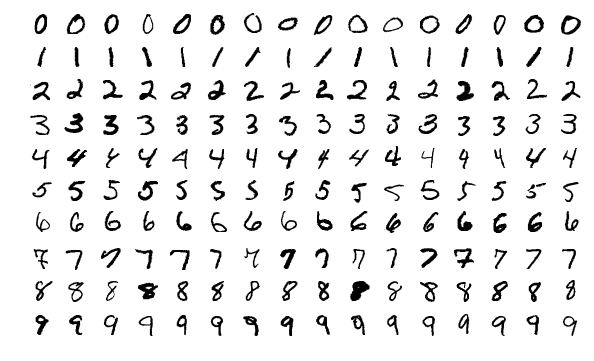
\includegraphics[width=0.75\textwidth]{img/MnistExamples.png}
		\caption{Esempio dei dati del MNIST (credits: Josef Steppan, Wikipedia)}
		\label{fig:mnistexamples}
	\end{center}
\end{figure}
\pagebreak

Per meglio comprendere i tre scenari proposti, i task relativi al dataset MNIST possono essere individuati nei seguenti:
\begin{itemize}
    \item[-] Task 1: identificare tra 0 e 1
    \item[-] Task 2: identificare tra 2 e 3
    \item[-] Task 3: identificare tra 4 e 5
    \item[-] Task 4: identificare tra 6 e 7
    \item[-] Task 5: identificare tra 8 e 9
\end{itemize}
Con questi task, i tre scenari individuati diventano:
\begin{itemize}
    \item[-] \textbf{Task-IL}: dato il task, è la prima o la seconda classe? Ad esempio, identificare fra 0 e 1
    \item[-] \textbf{Domain-IL}: senza sapere il task, è la prima o la seconda classe? Ad esempio, identificare se è un numero pari (prima classe) o dispari (seconda classe)
    \item[-] \textbf{Class-IL}: senza sapere il task, che cifra è? Nell'esempio, individuare quale cifra è da 0 a 9
\end{itemize}
\subsection{Reti Neurali Ricorrenti}
Una rete neurale ricorrente, o RNN, è una rete neurale dove i neuroni, o alcuni di essi, sono collegati a sé stessi in un ciclo chiuso. Questo collegamento consente ai layer di una RNN di mantenere informazioni in maniera analoga ad uno stato interno, permettendo di modellare, ad esempio, i comportamenti dinamici di una sequenza temporale fornita come input, dove ogni dato dipende anche dai dati precedenti già ricevuti.\\
In letteratura esistono diverse architetture di reti neurali ricorrenti, ma molte di esse devono la loro esistenza a due nodi ricorrenti fondamentali: le \textit{Long Short-Term Memory}, LSTM$^{\cite{10.1162/neco.1997.9.8.1735}}$, e le \textit{Gated Recurrent Unit}, GRU$^{\cite{DBLP:journals/corr/ChoMGBSB14}}$ (Figura \ref{fig:rnnlstmgru}). 
\begin{figure}[h]
	\begin{center}
		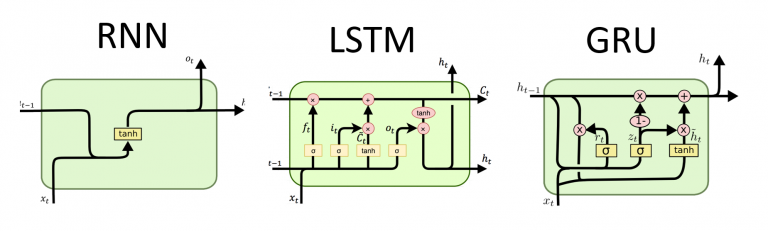
\includegraphics[width=0.95\textwidth]{img/rnnlstmgru.png}
		\caption{Schemi di nodi ricorrenti (credits: Michael Phi, towardsdatascience.com)}
		\label{fig:rnnlstmgru}
	\end{center}
\end{figure}
LSTM e GRU hanno meccanismi interni, chiamati \textit{gates} o cancelli, che regolano il flusso delle informazioni. Attraverso questi \textit{gate}, le unità apprendono quali dati sono importanti all'interno della sequenza e quali si possono ignorare, lasciando così al resto della rete solamente le informazioni che ritiene essere rilevanti per fare predizioni.\\\\
In una LSTM, i dati passano attraverso il \textit{forget gate}, che decide immediatamente quali informazioni è utile mantenere e quali ignorare. Dopodiché i dati passano attraverso l'\textit{input gate} assieme allo stato precedente dell'unità, che decide quali valori dello stato interno conviene aggiornare, e queste informazioni sono poi usate per aggiornare lo stato dell'unità. Infine, attraverso l'\textit{output gate} viene calcolato il nuovo stato interno dell'unità, che servirà all'input successivo.\\\\
Nelle GRU abbiamo un comportamento simile, ma la struttura dell'unità è semplificata. I dati passano subito attraverso il \textit{update gate}, che si comporta in modo simile ai \textit{gate} \textit{forget} e \textit{input} dell'LSTM, decidendo quali informazioni ignorare e quali mantenere. Dopodiché si attraversa il \textit{reset gate}, che decide cosa mantenere delle informazioni precedententemente analizzate. Avendo una struttura più semplificata, la GRU sono solitamente più veloci delle LSTM.
\subsection{Software e Hardware}
Negli ultimi anni sono nate diverse librerie software che consentono di realizzare modelli di Machine Learning performanti in breve tempo dei tipi più disparati, da semplici modelli lineari a reti neurali profonde convolutive e oltre.\\
Librerie open source come PyTorch, Tensorflow$^{\cite{abadi2016tensorflow}}$ e Keras, ma anche librerie proprietarie come Apple Core ML, IBM Watson e MATLAB Deep Learning Toolbox, hanno aperto le porte del Machine Learning a chiunque sia disposto a studiarle. Alcune librerie, come in particolare TensorFlow 2.0, possiedono API estremamente semplici che consentono di eseguire il preprocessing dei dataset, strutturare una rete neurale, addestrarla e valutarla con poche di righe di codice, e nonostante la semplicità essa consente comunque di mettere mano e andare a personalizzare ogni minimo aspetto di tutte le fasi, dal preprocessing al training. In letteratura sono disponibili anche moltissimi testi che consentono di approcciarsi facilmente al Machine Learning$^{\cite{chollet},\cite{geron}}$.\\\\
Anche a livello hardware gli ultimi anni hanno portato enormi sviluppi, grazie soprattutto all'industria videoludica e alle criptovalute che hanno spinto la ricerca e lo sviluppo di processori specializzati in calcolo parallelo e matriciale. Questi dispositivi, denominati \textit{Graphics Processing Unit} o GPU, consentono di ridurre esponenzialmente i tempi di addestramento delle reti neurali, abbassando ancora di più i requisiti per accedere a questo campo di studi e consentendo l'esecuzione di modelli di Machine Learning anche su un comune computer casalingo.\\
Inoltre, aziende come Google hanno sviluppato hardware realizzato ad hoc per le computazioni necessarie alle reti neurali, incrementando così ulteriormente la velocità e l'efficienza di questi modelli. Nel caso di Google, questo hardware è chiamato \textit{Tensor Processing Unit} o TPU.
\subsection{Applicazioni Future}
Alla luce degli attuali studi nell'ampio campo che è il Machine Learning, e in particolare riguardanti il continual learning e lo HSM, diventa chiaro come il futuro richiederà sempre più responsività ai sistemi predittivi e un sempre maggior grado di adattamento allo stato psico-fisico del momento dell'utente. Questa necessità di continua evoluzione ben si sposa con le caratteristiche del continual learning, e possibili applicazioni di questa sinergia continual learning -- HSM si possono individuare in diversi contesti, tra cui ad esempio:
\begin{itemize}
    \item[-] \textbf{Guida autonoma}.\\La crescente industria dei veicoli a guida autonoma ha portato ad uno sviluppo in moltissimi campi del Machine Learning$^{\cite{huang2020autonomous}}$, in particolare nel campo dell'\textit{object recognition}$^{\cite{Carranza_Garc_a_2021}}$, del \textit{behavioral planning}$^{\cite{6856582}}$ e altri ancora. L'\textit{autonomous driving} negli ultimi anni è, senza dubbio, uno dei motori principali nello sviluppo della disciplina del Machine Learning.\\
    Un veicolo a guida autonoma che sappia adattarsi allo stato psico-fisico attuale del conducente può portare a grossi benefici: ad esempio, essere in grado di modificare il proprio andamento per accomodare uno stato di malessere mitigando così il rischio di incidenti, o poter proporre tappe durante il percorso a seconda della condizione dei passeggeri portando così a più piacevole utilizzo del sistema da parte degli utenti.
    \item[-] \textbf{Intrattenimento}.\\L'industria dell'intrattenimento si è sempre interessata alle nuove tecnologie, puntando alla novità del momento in modo da raggiungere un pubblico sempre più ampio: ad esempio, la tecnologia degli schermi 3D o della realtà virtuale.\\
    Un sistema adattivo di riconoscimento dello stato psico-fisico dello spettatore o del videogiocatore può portare a esperienze multimediali più realistici e responsivi, che ad esempio possano adattare la propria narrazione o l'atmosfera proposta all'utente in maniera da sfruttare, o alleviare, eventuali emozioni che nascono nello spettatore.
    %\item[-] TODO altri esempi: interfacce che si modulano in base allo stato mentale del momento?
\end{itemize}
In tutti questi ambiti, per poter ottenere ottimi risultati, i sistemi devono essere in grado di adattarsi e specializzarsi nel riconoscere lo stato psico-fisico del singolo utente (ad esempio, il conducente proprietario del veicolo o il videogiocatore che possiede la console) ottenendo così sistemi calibrati e personalizzati in base alle caratteristiche e alle esigenze del singolo utente.\\\\
Questa sinergia risulta ancora poco studiata in letteratura, quindi può essere utile mettere sotto esame alcune tecniche di Addestramento Continuo attualmente studiate per giudicare la loro applicabilità o meno in contesti di \textit{Human State Monitoring}, così da concludere se siano necessari ulteriori sforzi in questa direzione per poter realizzare, in futuro, sistemi sempre più integrati con l'uomo e interfacce uomo-macchina sempre più intuitive e adattive. Valutare fin da subito l'applicabilità di questa sinergia è fondamentale in un campo di studi che si muove così in fretta come quello del Machine Learning.

